\documentclass[12pt]{article}
 
\usepackage[utf8x]{inputenc}
\usepackage[brazilian]{babel}
\usepackage{fontenc}
\usepackage{graphicx} 
\usepackage{listings}
\usepackage{xcolor}
\usepackage{indentfirst}
\usepackage{pdflscape}
\usepackage[bottom=3cm,top=3cm,left=3cm,right=3cm]{geometry} 
\usepackage[pdftex]{hyperref} %permitir \url

\usepackage{wallpaper}
\usepackage{subfig}

\usepackage{fancyhdr}
\pagestyle{fancy}
\fancyhf{}
\rhead{QXCode}
\lhead{Blackjack}
\fancyfoot[R]{\thepage}
%\rfoot{Page \thepage}


\usepackage[absolute]{textpos}


\lstset{
    language=java,
%    language=c++,
    keywordstyle=\bfseries\ttfamily\color[rgb]{0,0,1},
    identifierstyle=\ttfamily,
    commentstyle=\color[rgb]{0.133,0.545,0.133},
    stringstyle=\ttfamily\color[rgb]{0.627,0.126,0.941},
    showstringspaces=false,
    basicstyle=\small,
    tabsize=2,
    breaklines=true,
    frame=single
}



\renewcommand{\tt}[1]{\lstinline|#1|}
\renewcommand{\bf}[1]{\textbf{#1}}


\begin{document}

\ThisULCornerWallPaper{1}{./imagens/header}

\begin{textblock}{15}(0.4, 0.4)
\noindent
\begin{center}
\LARGE{\bf{QXCode - Quixadá Coding Team}}\\
\large{\bf{Fundamentos de Programação}} \\
\large{\bf{\today}}
\end{center}
\end{textblock}

\title{\bf{Bingo e Gerador de Cartelas}}

\author{
David Sena \thanks{sena.ufc@gmail.com}
}

\date{}

\maketitle
\thispagestyle{empty}

%#################################################################
%#################################################################
%#################################################################
%#################################################################


\section{Instruções Gerais}
O objetivo desse trabalho é fazer um código
que simule um bingo e um gerador de cartelas. 

\begin{figure}[hf]
\centering
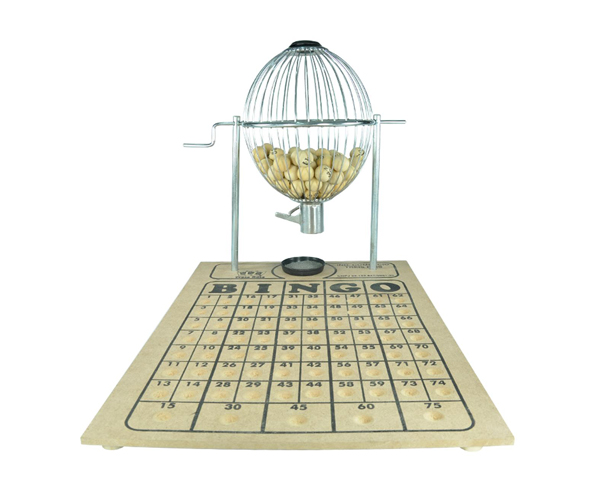
\includegraphics[width=0.8\linewidth]{./imagens/roleta}
\caption{Roleta e Mesa}
%\label{fig:blackjack}
\end{figure}

\url{http://www.bingosonline.com/regras-bingo/75-bolas}

\subsection{Regras Básicas}

O bingo de 75 bolas é a modalidade de bingo mais popular nos Estados Unidos. Esta tradicional variante do bingo utiliza 75 números, com grupos de 15. Cada letra da palavra "Bingo" é utilizada para agrupar 15 números, de 01 a 75. As cartelas do bingo de 75 bolas são quadaradas, com 25 espaços - 5 colunas e 5 linhas. O espaço que fica bem no centro da cartela é marcado com a palavra "Free" ("Livre"), ou seja, não será utilizado por nenhum jogador. Todos os demais espaços contem números aleatórios, dispostos conforme o layout "Bingo" anteriormente explicado, e devem ser preenchidos conforme são cantados.

Nesta modalidade de bingo, todos os jogadores devem preencher os espaços até completarem um padrão de preenchimento preestabelecido no início do jogo. Um padrão de linha requer que o jogador complete uma das linhas de sua cartela, o padrão X requer o preenchimento de duas linhas na diagonal, entre outros. O padrão "bingo" (todos os espaços completos) é conhecido nesta modalidade como "Full House", "Blackout", ou ainda "Coverall".

\section{Implementação Parte 1}
Seu objetivo é implementar a roleta e o rack de guardar as bolas.
A cada rodada, o programa pergunta pro usuário se quer pedir outra bola ou parar.
A cada bola sorteada, esta deve sair da roleta e ir para o rack.

Se programa deve continuamente mostrar quais as bolas que estão na roleta 
e quais as bolas que já foram sorteadas e estão no rack.

Como sugestão ordene esses valores para facilitar a visualização. Se desejar, 
implemente como no exemplo abaixo, no qual as bolas que faltam são mostradas
com um marcador.

\subsection{Exemplo}

1a Versão. Uma única rodada, um jogador e a mesa. A cada rodada o programa pergunta se o jogador quer para ou continuar. Se quiser continuar, recebe uma carta aleatória. Abaixo, um exemplo de saída.

\begin{verbatim}
Iniciando Bingo:

Roleta:
 1  2  3  4  5  6  7  8  9 10 11 12 13 14 15 
16 17 18 19 20 21 22 23 24 25 26 27 28 29 30 
31 32 33 34 35 36 37 38 39 40 41 42 43 44 45 
46 47 48 49 50 51 52 53 54 55 56 57 58 59 60 
61 62 63 64 65 66 67 68 69 70 71 72 73 74 75 
Escolha 1 para pedir bola e 0 para sair
>> 1

Numero sorteado 57

Roleta:
 1  2  3  4  5  6  7  8  9 10 11 12 13 14 15 
16 17 18 19 20 21 22 23 24 25 26 27 28 29 30 
31 32 33 34 35 36 37 38 39 40 41 42 43 44 45 
46 47 48 49 50 51 52 53 54 55 56 __ 58 59 60 
61 62 63 64 65 66 67 68 69 70 71 72 73 74 75 

Rack:
__ __ __ __ __ __ __ __ __ __ __ __ __ __ __ 
__ __ __ __ __ __ __ __ __ __ __ __ __ __ __ 
__ __ __ __ __ __ __ __ __ __ __ __ __ __ __ 
__ __ __ __ __ __ __ __ __ __ __ 57 __ __ __ 
__ __ __ __ __ __ __ __ __ __ __ __ __ __ __ 

Escolha 1 para pedir bola e 0 para sair
>> 1

Numero sorteado 58

Roleta:
 1  2  3  4  5  6  7  8  9 10 11 12 13 14 15 
16 17 18 19 20 21 22 23 24 25 26 27 28 29 30 
31 32 33 34 35 36 37 38 39 40 41 42 43 44 45 
46 47 48 49 50 51 52 53 54 55 56 __ __ 59 60 
61 62 63 64 65 66 67 68 69 70 71 72 73 74 75 

Rack:
__ __ __ __ __ __ __ __ __ __ __ __ __ __ __ 
__ __ __ __ __ __ __ __ __ __ __ __ __ __ __ 
__ __ __ __ __ __ __ __ __ __ __ __ __ __ __ 
__ __ __ __ __ __ __ __ __ __ __ 57 58 __ __ 
__ __ __ __ __ __ __ __ __ __ __ __ __ __ __ 
Escolha 1 para pedir bola e 0 para sair
>> 0

Obrigado e volte sempre.
\end{verbatim}


\subsection{Implementação Parte 2}
A segunda parte da implementação é a criação de um gerador de cartelas.
Aqui cada letra contem bolas dentro de uma faixa.
\begin{itemize}
\item B - 5 bolas entre 1 e 15
\item I - 5 bolas entre 16 e 30
\item N - 4 bolas entre 31 e 45
\item G - 5 bolas entre 46 e 60
\item O - 5 bolas entre 61 e 75
\end{itemize}


Os números normalmente não são ordenados dentro da letra. A seguir o exemplo de uma
cartela.

\begin{figure}[hf]
\centering
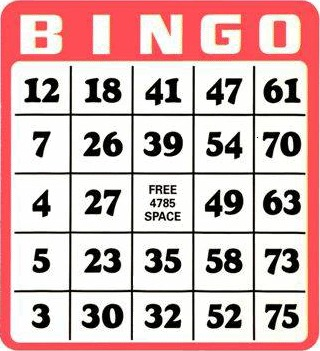
\includegraphics[width=0.6\linewidth]{./imagens/cartela}
\caption{Cartela}
%\label{fig:blackjack}
\end{figure}

\subsection{Exemplo Parte 2}

\begin{verbatim}


Cartela 1
B  I  N  G  O
12 18 31 58 63 
 3 19 43 54 67 
 1 26 ## 59 71 
10 23 45 50 68 
14 21 38 60 65 

Cartela 2
B  I  N  G  O
 4 17 43 50 67 
12 28 41 53 68 
 9 20 ## 59 72 
11 19 39 60 70 
13 16 37 48 62
\end{verbatim}

\begin{verbatim}


\end{verbatim}

\end{document}
